\section{Sub\-Bar\-Player Class Reference}
\label{classSubBarPlayer}\index{SubBarPlayer@{SubBarPlayer}}
{\tt \#include $<$subbarplayer.h$>$}

Inheritance diagram for Sub\-Bar\-Player:\begin{figure}[H]
\begin{center}
\leavevmode
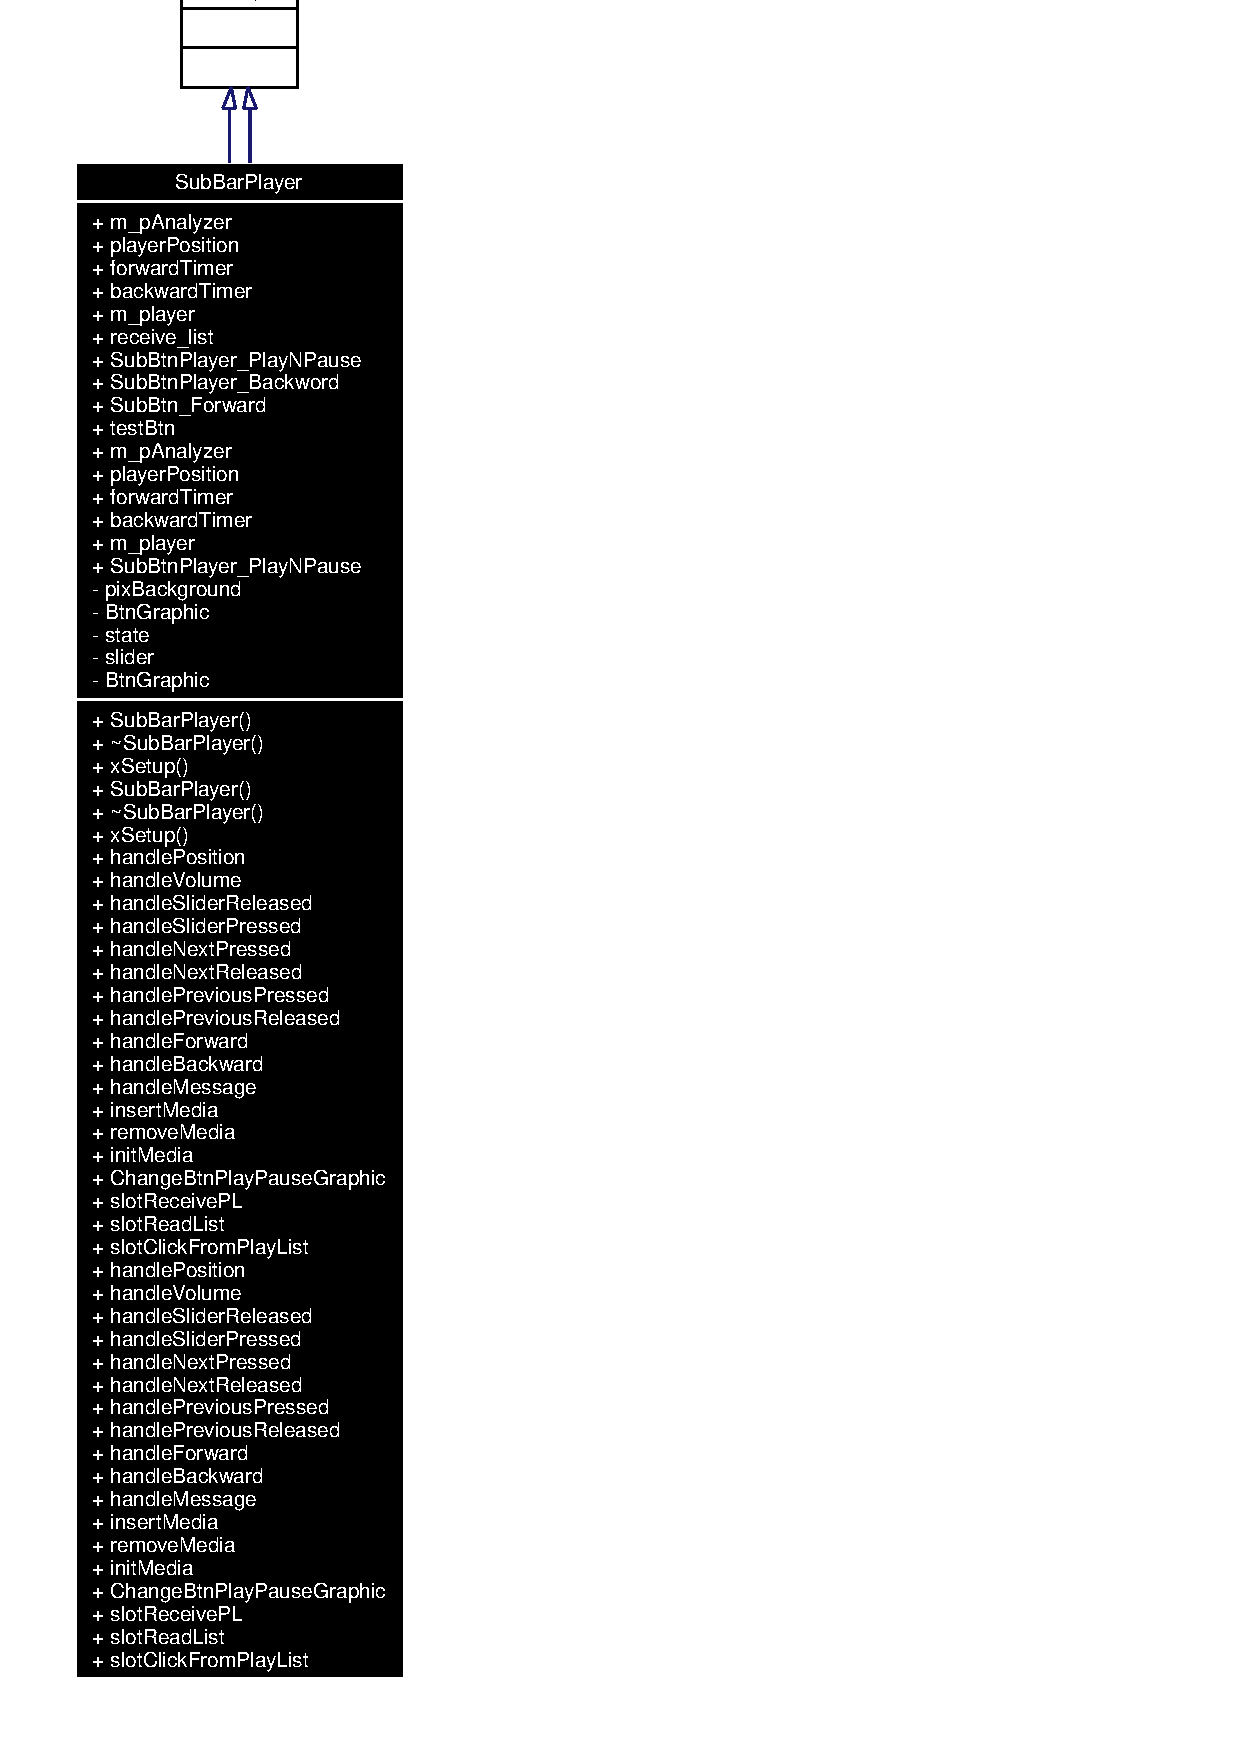
\includegraphics[width=97pt]{classSubBarPlayer__inherit__graph}
\end{center}
\end{figure}
Collaboration diagram for Sub\-Bar\-Player:\begin{figure}[H]
\begin{center}
\leavevmode
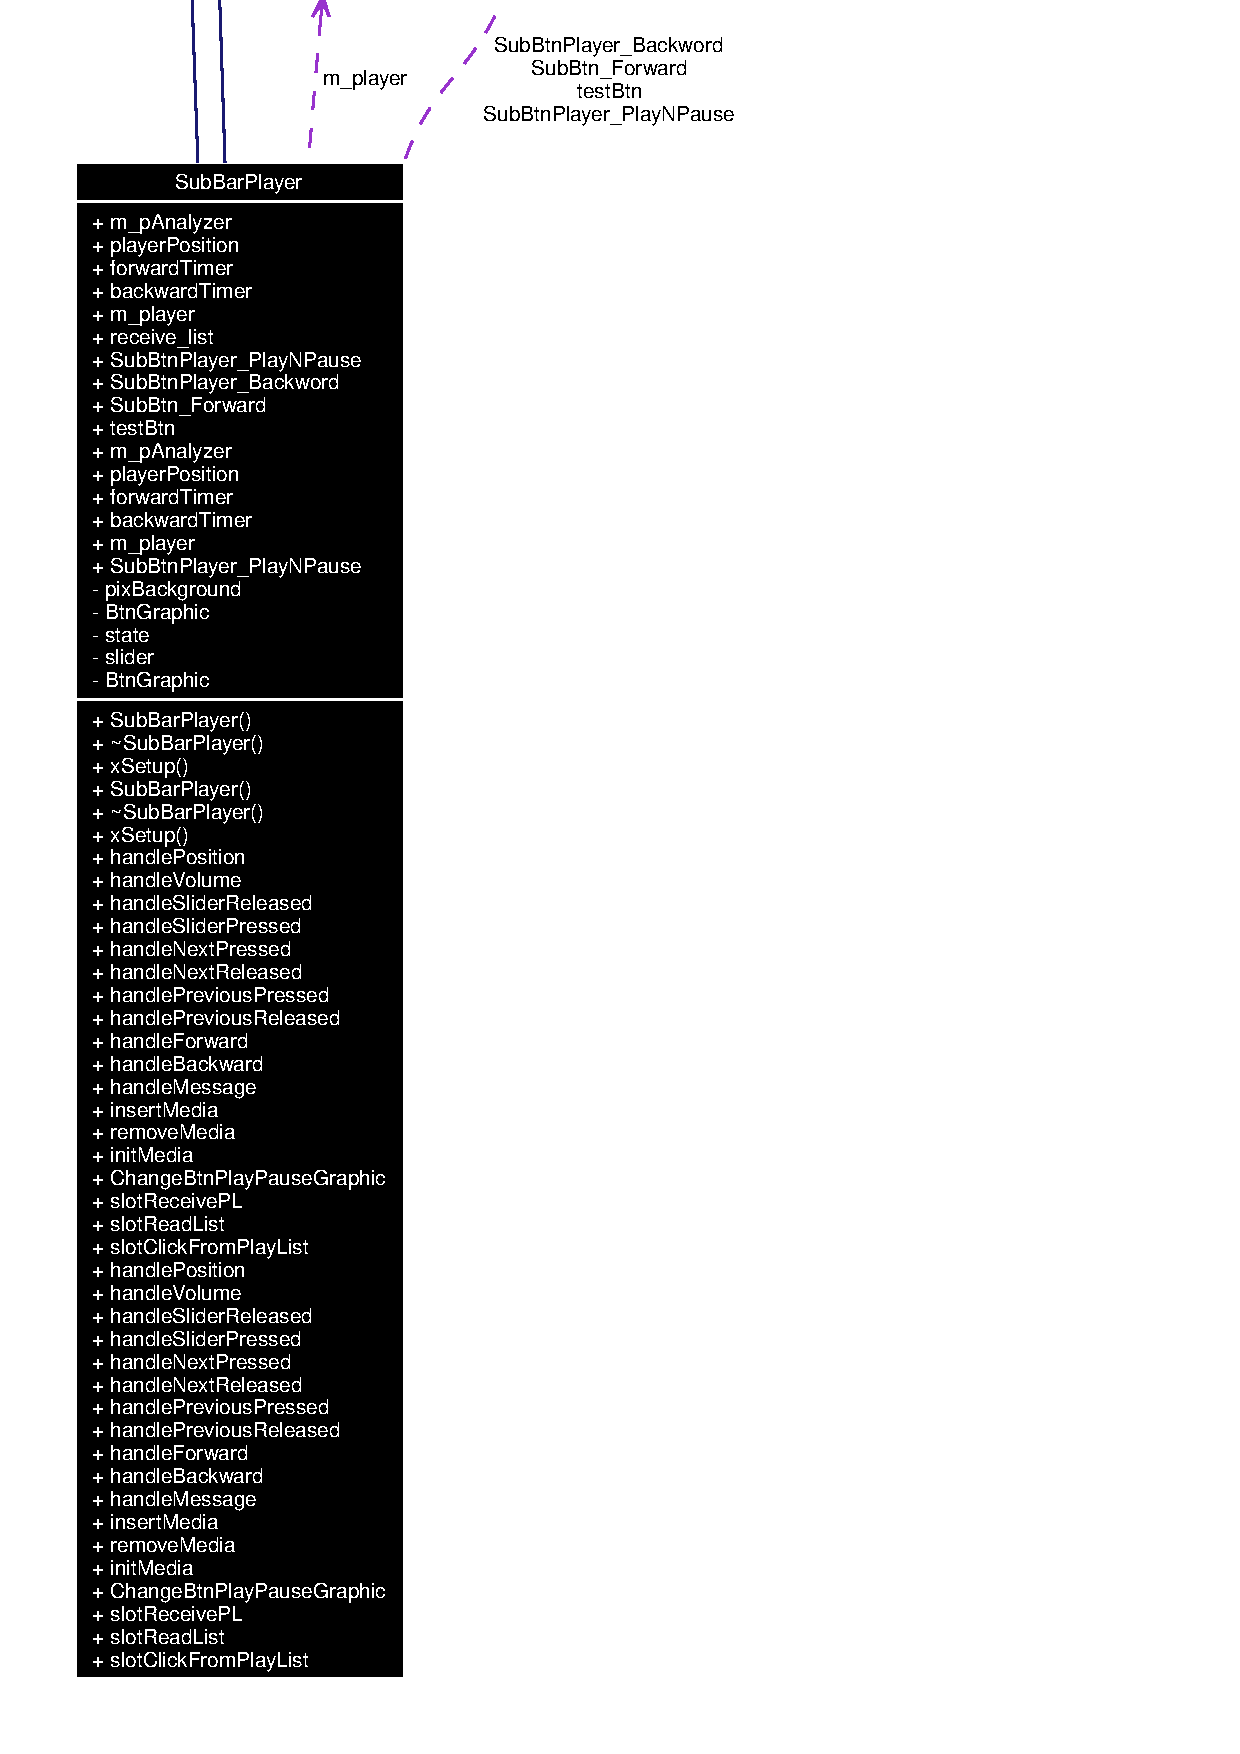
\includegraphics[width=203pt]{classSubBarPlayer__coll__graph}
\end{center}
\end{figure}


\subsection{Detailed Description}
\begin{Desc}
\item[Author:]sonicat \end{Desc}




Definition at line 39 of file src/subbarplayer.h.\subsection*{Public Slots}
\begin{CompactItemize}
\item 
void {\bf handle\-Position} (int)
\item 
void {\bf handle\-Volume} (int)
\item 
void {\bf handle\-Slider\-Released} ()
\item 
void {\bf handle\-Slider\-Pressed} ()
\item 
void {\bf handle\-Next\-Pressed} ()
\item 
void {\bf handle\-Next\-Released} ()
\item 
void {\bf handle\-Previous\-Pressed} ()
\item 
void {\bf handle\-Previous\-Released} ()
\item 
void {\bf handle\-Forward} ()
\item 
void {\bf handle\-Backward} ()
\item 
void {\bf handle\-Message} (int m\_\-length, int m\_\-bitrate, QString m\_\-title, QString m\_\-artist, QString m\_\-album)
\item 
void {\bf insert\-Media} (KURL::List list)
\item 
void {\bf remove\-Media} (KURL::List remove\_\-list)
\item 
void {\bf init\-Media} (KURL::List list)
\item 
void {\bf Change\-Btn\-Play\-Pause\-Graphic} ()
\item 
void {\bf slot\-Receive\-PL} (KURL::List list)
\item 
void {\bf slot\-Read\-List} ()
\item 
void {\bf slot\-Click\-From\-Play\-List} ()
\item 
void {\bf handle\-Position} (int)
\item 
void {\bf handle\-Volume} (int)
\item 
void {\bf handle\-Slider\-Released} ()
\item 
void {\bf handle\-Slider\-Pressed} ()
\item 
void {\bf handle\-Next\-Pressed} ()
\item 
void {\bf handle\-Next\-Released} ()
\item 
void {\bf handle\-Previous\-Pressed} ()
\item 
void {\bf handle\-Previous\-Released} ()
\item 
void {\bf handle\-Forward} ()
\item 
void {\bf handle\-Backward} ()
\item 
void {\bf handle\-Message} (int m\_\-length, int m\_\-bitrate, QString m\_\-title, QString m\_\-artist, QString m\_\-album)
\item 
void {\bf insert\-Media} (KURL::List list)
\item 
void {\bf remove\-Media} (KURL::List remove\_\-list)
\item 
void {\bf init\-Media} (KURL::List list)
\item 
void {\bf Change\-Btn\-Play\-Pause\-Graphic} ()
\item 
void {\bf slot\-Receive\-PL} (KURL::List list)
\item 
void {\bf slot\-Read\-List} ()
\item 
void {\bf slot\-Click\-From\-Play\-List} ()
\end{CompactItemize}
\subsection*{Signals}
\begin{CompactItemize}
\item 
void {\bf signal\-Request\-PL} ()
\item 
void {\bf signal\-Request\-PL} ()
\end{CompactItemize}
\subsection*{Public Member Functions}
\begin{CompactItemize}
\item 
{\bf Sub\-Bar\-Player} ({\bf QWidget} $\ast$parent=0, const char $\ast$name=0)
\item 
{\bf $\sim$Sub\-Bar\-Player} ()
\item 
void {\bf x\-Setup} ()
\item 
{\bf Sub\-Bar\-Player} ({\bf QWidget} $\ast$parent=0, const char $\ast$name=0)
\item 
{\bf $\sim$Sub\-Bar\-Player} ()
\item 
void {\bf x\-Setup} ()
\end{CompactItemize}
\subsection*{Public Attributes}
\begin{CompactItemize}
\item 
{\bf QWidget} $\ast$ {\bf m\_\-p\-Analyzer}
\item 
QSlider $\ast$ {\bf player\-Position}
\item 
QTimer $\ast$ {\bf forward\-Timer}
\item 
QTimer $\ast$ {\bf backward\-Timer}
\item 
{\bf Myplayer} $\ast$ {\bf m\_\-player}
\item 
KURL::List {\bf receive\_\-list}
\item 
{\bf Skin\-Button} $\ast$ {\bf Sub\-Btn\-Player\_\-Play\-NPause}
\item 
{\bf Skin\-Button} $\ast$ {\bf Sub\-Btn\-Player\_\-Backword}
\item 
{\bf Skin\-Button} $\ast$ {\bf Sub\-Btn\_\-Forward}
\item 
{\bf Skin\-Button} $\ast$ {\bf test\-Btn}
\item 
{\bf QWidget} $\ast$ {\bf m\_\-p\-Analyzer}
\item 
QSlider $\ast$ {\bf player\-Position}
\item 
QTimer $\ast$ {\bf forward\-Timer}
\item 
QTimer $\ast$ {\bf backward\-Timer}
\item 
{\bf Myplayer} $\ast$ {\bf m\_\-player}
\item 
{\bf Skin\-Button} $\ast$ {\bf Sub\-Btn\-Player\_\-Play\-NPause}
\end{CompactItemize}
\subsection*{Private Types}
\begin{CompactItemize}
\item 
enum {\bf PLAYSTATE} \{ {\bf PAUSE}, 
{\bf GO}
 \}
\item 
enum {\bf PLAYSTATE} \{ {\bf PAUSE}, 
{\bf GO}
 \}
\end{CompactItemize}
\subsection*{Private Attributes}
\begin{CompactItemize}
\item 
QPixmap {\bf pix\-Background}
\item 
QPixmap $\ast$ {\bf Btn\-Graphic} [8]
\item 
{\bf PLAYSTATE} {\bf state}
\item 
bool {\bf slider}
\item 
QPixmap $\ast$ {\bf Btn\-Graphic} [8]
\end{CompactItemize}


\subsection{Member Enumeration Documentation}
\index{SubBarPlayer@{Sub\-Bar\-Player}!PLAYSTATE@{PLAYSTATE}}
\index{PLAYSTATE@{PLAYSTATE}!SubBarPlayer@{Sub\-Bar\-Player}}
\subsubsection{\setlength{\rightskip}{0pt plus 5cm}enum {\bf Sub\-Bar\-Player::PLAYSTATE}\hspace{0.3cm}{\tt  [private]}}\label{classSubBarPlayer_SubBarPlayery3}


\begin{Desc}
\item[Enumeration values: ]\par
\begin{description}
\index{PAUSE@{PAUSE}!SubBarPlayer@{SubBarPlayer}}\index{SubBarPlayer@{SubBarPlayer}!PAUSE@{PAUSE}}\item[{\em 
PAUSE\label{classSubBarPlayer_SubBarPlayery3SubBarPlayery0}
}]\index{GO@{GO}!SubBarPlayer@{SubBarPlayer}}\index{SubBarPlayer@{SubBarPlayer}!GO@{GO}}\item[{\em 
GO\label{classSubBarPlayer_SubBarPlayery3SubBarPlayery1}
}]\end{description}
\end{Desc}



Definition at line 42 of file subbarplayer.h.



\footnotesize\begin{verbatim}42 {PAUSE,GO};
\end{verbatim}\normalsize 
\index{SubBarPlayer@{Sub\-Bar\-Player}!PLAYSTATE@{PLAYSTATE}}
\index{PLAYSTATE@{PLAYSTATE}!SubBarPlayer@{Sub\-Bar\-Player}}
\subsubsection{\setlength{\rightskip}{0pt plus 5cm}enum {\bf Sub\-Bar\-Player::PLAYSTATE}\hspace{0.3cm}{\tt  [private]}}\label{classSubBarPlayer_SubBarPlayery2}


\begin{Desc}
\item[Enumeration values: ]\par
\begin{description}
\index{PAUSE@{PAUSE}!SubBarPlayer@{SubBarPlayer}}\index{SubBarPlayer@{SubBarPlayer}!PAUSE@{PAUSE}}\item[{\em 
PAUSE\label{classSubBarPlayer_SubBarPlayery3SubBarPlayery0}
}]\index{GO@{GO}!SubBarPlayer@{SubBarPlayer}}\index{SubBarPlayer@{SubBarPlayer}!GO@{GO}}\item[{\em 
GO\label{classSubBarPlayer_SubBarPlayery3SubBarPlayery1}
}]\end{description}
\end{Desc}



Definition at line 42 of file src/subbarplayer.h.



\footnotesize\begin{verbatim}42 {PAUSE,GO};
\end{verbatim}\normalsize 


\subsection{Constructor \& Destructor Documentation}
\index{SubBarPlayer@{Sub\-Bar\-Player}!SubBarPlayer@{SubBarPlayer}}
\index{SubBarPlayer@{SubBarPlayer}!SubBarPlayer@{Sub\-Bar\-Player}}
\subsubsection{\setlength{\rightskip}{0pt plus 5cm}Sub\-Bar\-Player::Sub\-Bar\-Player ({\bf QWidget} $\ast$ {\em parent} = 0, const char $\ast$ {\em name} = 0)}\label{classSubBarPlayer_SubBarPlayera0}




Definition at line 22 of file src/subbarplayer.cpp.

References m\_\-player, slider, and x\-Setup().



\footnotesize\begin{verbatim}23  : QWidget(parent, name)
24 {
25   //new Player here
26   m_player=new Myplayer;
27  
28   slider = true;
29   xSetup();
30 }
\end{verbatim}\normalsize 


Here is the call graph for this function:\begin{figure}[H]
\begin{center}
\leavevmode
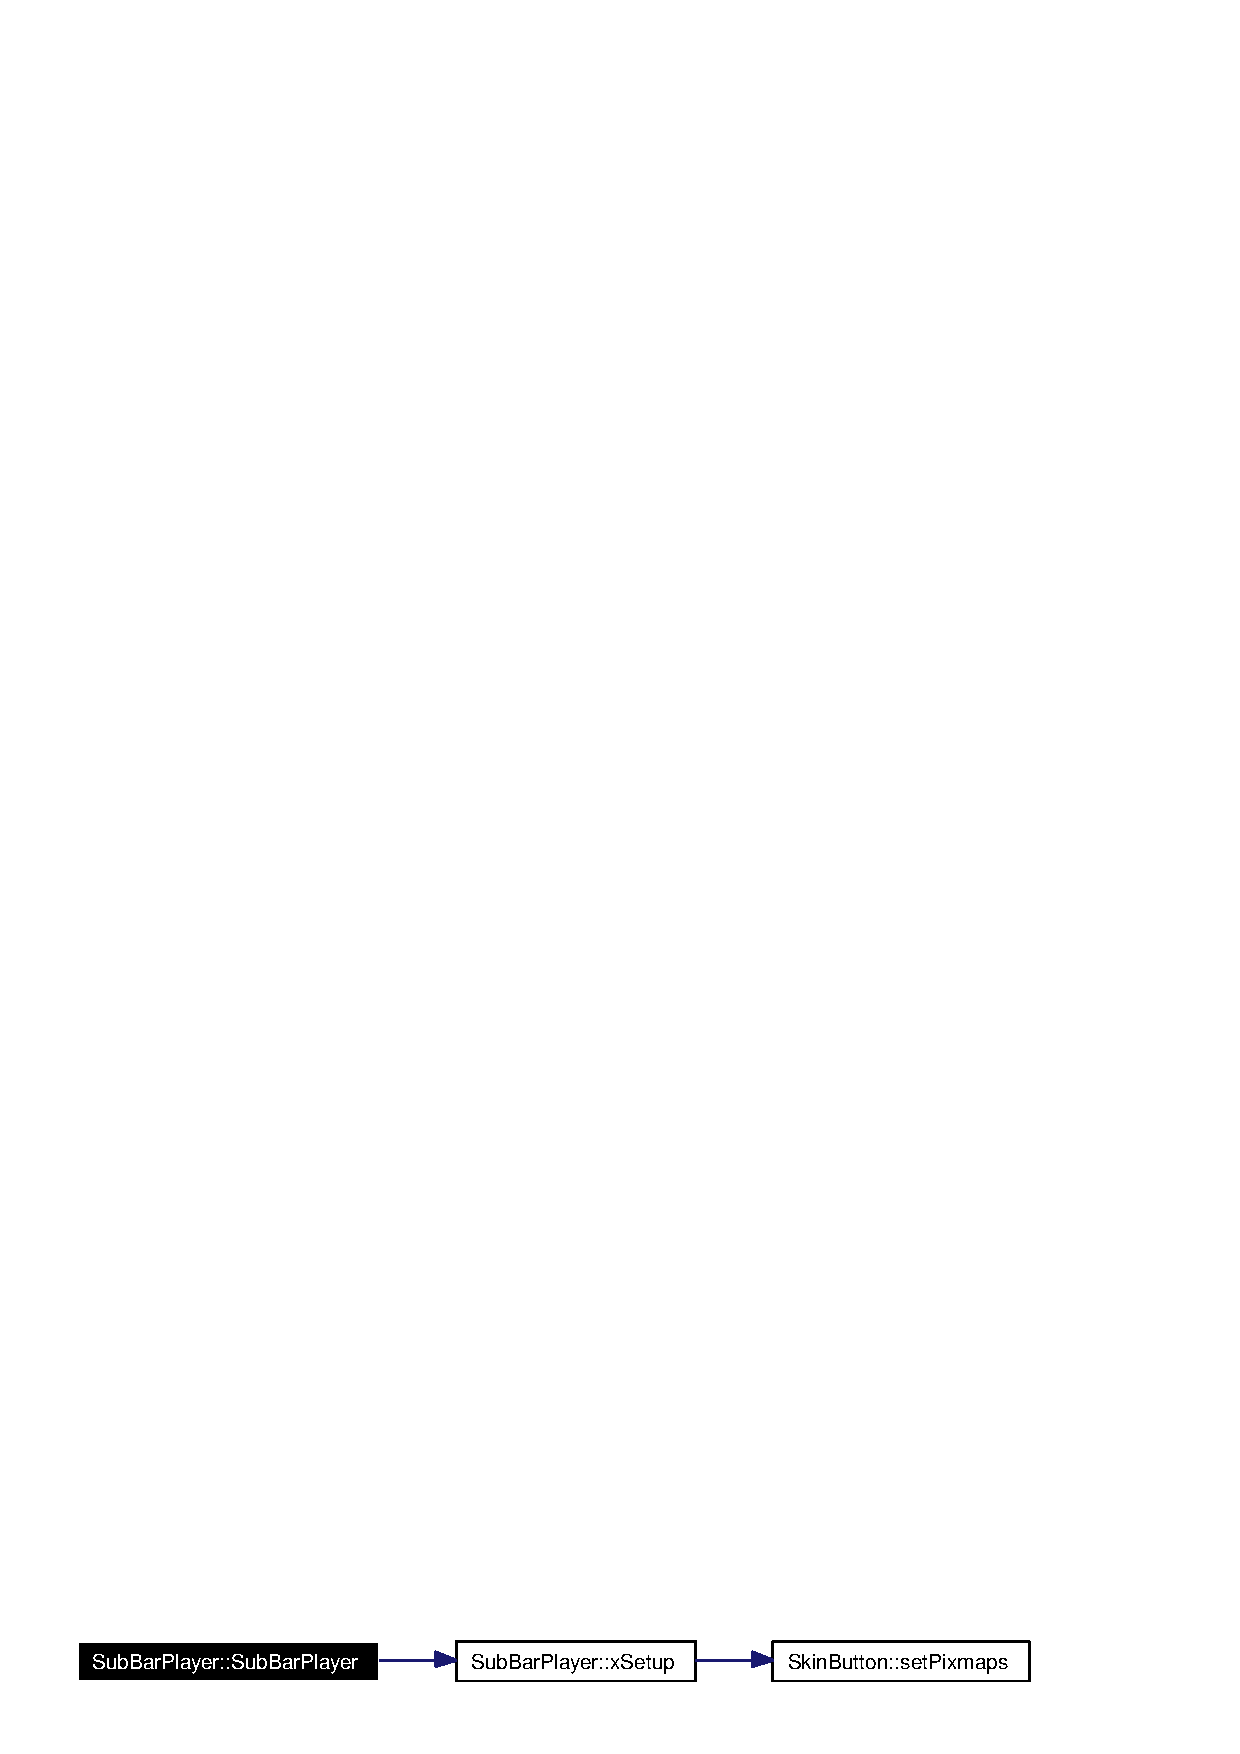
\includegraphics[width=247pt]{classSubBarPlayer_SubBarPlayera0_cgraph}
\end{center}
\end{figure}
\index{SubBarPlayer@{Sub\-Bar\-Player}!~SubBarPlayer@{$\sim$SubBarPlayer}}
\index{~SubBarPlayer@{$\sim$SubBarPlayer}!SubBarPlayer@{Sub\-Bar\-Player}}
\subsubsection{\setlength{\rightskip}{0pt plus 5cm}Sub\-Bar\-Player::$\sim${\bf Sub\-Bar\-Player} ()}\label{classSubBarPlayer_SubBarPlayera1}




Definition at line 33 of file src/subbarplayer.cpp.

References m\_\-player.



\footnotesize\begin{verbatim}34 {
35   delete m_player;
36 }
\end{verbatim}\normalsize 
\index{SubBarPlayer@{Sub\-Bar\-Player}!SubBarPlayer@{SubBarPlayer}}
\index{SubBarPlayer@{SubBarPlayer}!SubBarPlayer@{Sub\-Bar\-Player}}
\subsubsection{\setlength{\rightskip}{0pt plus 5cm}Sub\-Bar\-Player::Sub\-Bar\-Player ({\bf QWidget} $\ast$ {\em parent} = 0, const char $\ast$ {\em name} = 0)}\label{classSubBarPlayer_SubBarPlayera3}


\index{SubBarPlayer@{Sub\-Bar\-Player}!~SubBarPlayer@{$\sim$SubBarPlayer}}
\index{~SubBarPlayer@{$\sim$SubBarPlayer}!SubBarPlayer@{Sub\-Bar\-Player}}
\subsubsection{\setlength{\rightskip}{0pt plus 5cm}Sub\-Bar\-Player::$\sim${\bf Sub\-Bar\-Player} ()}\label{classSubBarPlayer_SubBarPlayera4}




\subsection{Member Function Documentation}
\index{SubBarPlayer@{Sub\-Bar\-Player}!ChangeBtnPlayPauseGraphic@{ChangeBtnPlayPauseGraphic}}
\index{ChangeBtnPlayPauseGraphic@{ChangeBtnPlayPauseGraphic}!SubBarPlayer@{Sub\-Bar\-Player}}
\subsubsection{\setlength{\rightskip}{0pt plus 5cm}void Sub\-Bar\-Player::Change\-Btn\-Play\-Pause\-Graphic ()\hspace{0.3cm}{\tt  [slot]}}\label{classSubBarPlayer_SubBarPlayeri32}


\index{SubBarPlayer@{Sub\-Bar\-Player}!ChangeBtnPlayPauseGraphic@{ChangeBtnPlayPauseGraphic}}
\index{ChangeBtnPlayPauseGraphic@{ChangeBtnPlayPauseGraphic}!SubBarPlayer@{Sub\-Bar\-Player}}
\subsubsection{\setlength{\rightskip}{0pt plus 5cm}void Sub\-Bar\-Player::Change\-Btn\-Play\-Pause\-Graphic ()\hspace{0.3cm}{\tt  [slot]}}\label{classSubBarPlayer_SubBarPlayeri14}




Definition at line 99 of file src/subbarplayer.cpp.

References GO, PAUSE, Skin\-Button::set\-Pixmaps(), and Sub\-Btn\-Player\_\-Play\-NPause.

Referenced by slot\-Click\-From\-Play\-List(), and x\-Setup().



\footnotesize\begin{verbatim}100 {
101   if(state==SubBarPlayer::PAUSE)
102   {
103     state=SubBarPlayer::GO;
104     SubBtnPlayer_PlayNPause->setPixmaps(BtnGraphic[2],BtnGraphic[3]);
105   }
106   else
107   {
108     state=SubBarPlayer::PAUSE;
109     SubBtnPlayer_PlayNPause->setPixmaps(BtnGraphic[4],BtnGraphic[5]);
110   }
111 }
\end{verbatim}\normalsize 
\index{SubBarPlayer@{Sub\-Bar\-Player}!handleBackward@{handleBackward}}
\index{handleBackward@{handleBackward}!SubBarPlayer@{Sub\-Bar\-Player}}
\subsubsection{\setlength{\rightskip}{0pt plus 5cm}void Sub\-Bar\-Player::handle\-Backward ()\hspace{0.3cm}{\tt  [slot]}}\label{classSubBarPlayer_SubBarPlayeri27}


\index{SubBarPlayer@{Sub\-Bar\-Player}!handleBackward@{handleBackward}}
\index{handleBackward@{handleBackward}!SubBarPlayer@{Sub\-Bar\-Player}}
\subsubsection{\setlength{\rightskip}{0pt plus 5cm}void Sub\-Bar\-Player::handle\-Backward ()\hspace{0.3cm}{\tt  [slot]}}\label{classSubBarPlayer_SubBarPlayeri9}




Definition at line 195 of file src/subbarplayer.cpp.

References player\-Position.

Referenced by x\-Setup().



\footnotesize\begin{verbatim}196 {
197      kdDebug() << "[UI::handleBackward]" << endl;
198      int fast = playerPosition->value();
199      fast--;
200      playerPosition->setValue(fast);
201 }
\end{verbatim}\normalsize 
\index{SubBarPlayer@{Sub\-Bar\-Player}!handleForward@{handleForward}}
\index{handleForward@{handleForward}!SubBarPlayer@{Sub\-Bar\-Player}}
\subsubsection{\setlength{\rightskip}{0pt plus 5cm}void Sub\-Bar\-Player::handle\-Forward ()\hspace{0.3cm}{\tt  [slot]}}\label{classSubBarPlayer_SubBarPlayeri26}


\index{SubBarPlayer@{Sub\-Bar\-Player}!handleForward@{handleForward}}
\index{handleForward@{handleForward}!SubBarPlayer@{Sub\-Bar\-Player}}
\subsubsection{\setlength{\rightskip}{0pt plus 5cm}void Sub\-Bar\-Player::handle\-Forward ()\hspace{0.3cm}{\tt  [slot]}}\label{classSubBarPlayer_SubBarPlayeri8}




Definition at line 171 of file src/subbarplayer.cpp.

References player\-Position.

Referenced by x\-Setup().



\footnotesize\begin{verbatim}172 {
173      kdDebug() << "[UI::handleForward]" << endl;
174      int fast = playerPosition->value();
175      fast++;
176      playerPosition->setValue(fast);
177 //     Pos->setNum(fast);
178 }
\end{verbatim}\normalsize 
\index{SubBarPlayer@{Sub\-Bar\-Player}!handleMessage@{handleMessage}}
\index{handleMessage@{handleMessage}!SubBarPlayer@{Sub\-Bar\-Player}}
\subsubsection{\setlength{\rightskip}{0pt plus 5cm}void Sub\-Bar\-Player::handle\-Message (int {\em m\_\-length}, int {\em m\_\-bitrate}, QString {\em m\_\-title}, QString {\em m\_\-artist}, QString {\em m\_\-album})\hspace{0.3cm}{\tt  [slot]}}\label{classSubBarPlayer_SubBarPlayeri28}


\index{SubBarPlayer@{Sub\-Bar\-Player}!handleMessage@{handleMessage}}
\index{handleMessage@{handleMessage}!SubBarPlayer@{Sub\-Bar\-Player}}
\subsubsection{\setlength{\rightskip}{0pt plus 5cm}void Sub\-Bar\-Player::handle\-Message (int {\em m\_\-length}, int {\em m\_\-bitrate}, QString {\em m\_\-title}, QString {\em m\_\-artist}, QString {\em m\_\-album})\hspace{0.3cm}{\tt  [slot]}}\label{classSubBarPlayer_SubBarPlayeri10}




Definition at line 203 of file src/subbarplayer.cpp.

References player\-Position.

Referenced by x\-Setup().



\footnotesize\begin{verbatim}204 {
205         playerPosition->setMaxValue(m_length);
206 }
\end{verbatim}\normalsize 
\index{SubBarPlayer@{Sub\-Bar\-Player}!handleNextPressed@{handleNextPressed}}
\index{handleNextPressed@{handleNextPressed}!SubBarPlayer@{Sub\-Bar\-Player}}
\subsubsection{\setlength{\rightskip}{0pt plus 5cm}void Sub\-Bar\-Player::handle\-Next\-Pressed ()\hspace{0.3cm}{\tt  [slot]}}\label{classSubBarPlayer_SubBarPlayeri22}


\index{SubBarPlayer@{Sub\-Bar\-Player}!handleNextPressed@{handleNextPressed}}
\index{handleNextPressed@{handleNextPressed}!SubBarPlayer@{Sub\-Bar\-Player}}
\subsubsection{\setlength{\rightskip}{0pt plus 5cm}void Sub\-Bar\-Player::handle\-Next\-Pressed ()\hspace{0.3cm}{\tt  [slot]}}\label{classSubBarPlayer_SubBarPlayeri4}




Definition at line 155 of file src/subbarplayer.cpp.

References forward\-Timer, and slider.



\footnotesize\begin{verbatim}156 {
157      kdDebug() << "Next Pressed"<< endl;
158      forwardTimer->start( 100 );
159      slider = false;
160      
161 }
\end{verbatim}\normalsize 
\index{SubBarPlayer@{Sub\-Bar\-Player}!handleNextReleased@{handleNextReleased}}
\index{handleNextReleased@{handleNextReleased}!SubBarPlayer@{Sub\-Bar\-Player}}
\subsubsection{\setlength{\rightskip}{0pt plus 5cm}void Sub\-Bar\-Player::handle\-Next\-Released ()\hspace{0.3cm}{\tt  [slot]}}\label{classSubBarPlayer_SubBarPlayeri23}


\index{SubBarPlayer@{Sub\-Bar\-Player}!handleNextReleased@{handleNextReleased}}
\index{handleNextReleased@{handleNextReleased}!SubBarPlayer@{Sub\-Bar\-Player}}
\subsubsection{\setlength{\rightskip}{0pt plus 5cm}void Sub\-Bar\-Player::handle\-Next\-Released ()\hspace{0.3cm}{\tt  [slot]}}\label{classSubBarPlayer_SubBarPlayeri5}




Definition at line 163 of file src/subbarplayer.cpp.

References forward\-Timer, Myplayer::handle\-Slider(), m\_\-player, player\-Position, and slider.



\footnotesize\begin{verbatim}164 {
165      kdDebug() << "Next Released" << endl;
166      forwardTimer->stop();
167      m_player->handleSlider(playerPosition->value());
168      slider = true;
169 }
\end{verbatim}\normalsize 
\index{SubBarPlayer@{Sub\-Bar\-Player}!handlePosition@{handlePosition}}
\index{handlePosition@{handlePosition}!SubBarPlayer@{Sub\-Bar\-Player}}
\subsubsection{\setlength{\rightskip}{0pt plus 5cm}void Sub\-Bar\-Player::handle\-Position (int)\hspace{0.3cm}{\tt  [slot]}}\label{classSubBarPlayer_SubBarPlayeri18}


\index{SubBarPlayer@{Sub\-Bar\-Player}!handlePosition@{handlePosition}}
\index{handlePosition@{handlePosition}!SubBarPlayer@{Sub\-Bar\-Player}}
\subsubsection{\setlength{\rightskip}{0pt plus 5cm}void Sub\-Bar\-Player::handle\-Position (int)\hspace{0.3cm}{\tt  [slot]}}\label{classSubBarPlayer_SubBarPlayeri0}




Definition at line 134 of file src/subbarplayer.cpp.

References player\-Position, and slider.

Referenced by x\-Setup().



\footnotesize\begin{verbatim}135 {
136 
137      if(slider)playerPosition->setValue(position);    
138 }
\end{verbatim}\normalsize 
\index{SubBarPlayer@{Sub\-Bar\-Player}!handlePreviousPressed@{handlePreviousPressed}}
\index{handlePreviousPressed@{handlePreviousPressed}!SubBarPlayer@{Sub\-Bar\-Player}}
\subsubsection{\setlength{\rightskip}{0pt plus 5cm}void Sub\-Bar\-Player::handle\-Previous\-Pressed ()\hspace{0.3cm}{\tt  [slot]}}\label{classSubBarPlayer_SubBarPlayeri24}


\index{SubBarPlayer@{Sub\-Bar\-Player}!handlePreviousPressed@{handlePreviousPressed}}
\index{handlePreviousPressed@{handlePreviousPressed}!SubBarPlayer@{Sub\-Bar\-Player}}
\subsubsection{\setlength{\rightskip}{0pt plus 5cm}void Sub\-Bar\-Player::handle\-Previous\-Pressed ()\hspace{0.3cm}{\tt  [slot]}}\label{classSubBarPlayer_SubBarPlayeri6}




Definition at line 180 of file src/subbarplayer.cpp.

References backward\-Timer, and slider.



\footnotesize\begin{verbatim}181 {
182      kdDebug() << "Previous Pressed"<< endl;
183      backwardTimer->start( 100 );
184      slider = false;
185 }
\end{verbatim}\normalsize 
\index{SubBarPlayer@{Sub\-Bar\-Player}!handlePreviousReleased@{handlePreviousReleased}}
\index{handlePreviousReleased@{handlePreviousReleased}!SubBarPlayer@{Sub\-Bar\-Player}}
\subsubsection{\setlength{\rightskip}{0pt plus 5cm}void Sub\-Bar\-Player::handle\-Previous\-Released ()\hspace{0.3cm}{\tt  [slot]}}\label{classSubBarPlayer_SubBarPlayeri25}


\index{SubBarPlayer@{Sub\-Bar\-Player}!handlePreviousReleased@{handlePreviousReleased}}
\index{handlePreviousReleased@{handlePreviousReleased}!SubBarPlayer@{Sub\-Bar\-Player}}
\subsubsection{\setlength{\rightskip}{0pt plus 5cm}void Sub\-Bar\-Player::handle\-Previous\-Released ()\hspace{0.3cm}{\tt  [slot]}}\label{classSubBarPlayer_SubBarPlayeri7}




Definition at line 187 of file src/subbarplayer.cpp.

References backward\-Timer, Myplayer::handle\-Slider(), m\_\-player, player\-Position, and slider.



\footnotesize\begin{verbatim}188 {
189      kdDebug() << "Previous Released" << endl;
190      backwardTimer->stop();
191      m_player->handleSlider(playerPosition->value());
192      slider = true;
193 }
\end{verbatim}\normalsize 
\index{SubBarPlayer@{Sub\-Bar\-Player}!handleSliderPressed@{handleSliderPressed}}
\index{handleSliderPressed@{handleSliderPressed}!SubBarPlayer@{Sub\-Bar\-Player}}
\subsubsection{\setlength{\rightskip}{0pt plus 5cm}void Sub\-Bar\-Player::handle\-Slider\-Pressed ()\hspace{0.3cm}{\tt  [slot]}}\label{classSubBarPlayer_SubBarPlayeri21}


\index{SubBarPlayer@{Sub\-Bar\-Player}!handleSliderPressed@{handleSliderPressed}}
\index{handleSliderPressed@{handleSliderPressed}!SubBarPlayer@{Sub\-Bar\-Player}}
\subsubsection{\setlength{\rightskip}{0pt plus 5cm}void Sub\-Bar\-Player::handle\-Slider\-Pressed ()\hspace{0.3cm}{\tt  [slot]}}\label{classSubBarPlayer_SubBarPlayeri3}




Definition at line 150 of file src/subbarplayer.cpp.

References slider.

Referenced by x\-Setup().



\footnotesize\begin{verbatim}151 {
152      slider = false;
153 }
\end{verbatim}\normalsize 
\index{SubBarPlayer@{Sub\-Bar\-Player}!handleSliderReleased@{handleSliderReleased}}
\index{handleSliderReleased@{handleSliderReleased}!SubBarPlayer@{Sub\-Bar\-Player}}
\subsubsection{\setlength{\rightskip}{0pt plus 5cm}void Sub\-Bar\-Player::handle\-Slider\-Released ()\hspace{0.3cm}{\tt  [slot]}}\label{classSubBarPlayer_SubBarPlayeri20}


\index{SubBarPlayer@{Sub\-Bar\-Player}!handleSliderReleased@{handleSliderReleased}}
\index{handleSliderReleased@{handleSliderReleased}!SubBarPlayer@{Sub\-Bar\-Player}}
\subsubsection{\setlength{\rightskip}{0pt plus 5cm}void Sub\-Bar\-Player::handle\-Slider\-Released ()\hspace{0.3cm}{\tt  [slot]}}\label{classSubBarPlayer_SubBarPlayeri2}




Definition at line 144 of file src/subbarplayer.cpp.

References Myplayer::handle\-Slider(), m\_\-player, player\-Position, and slider.

Referenced by x\-Setup().



\footnotesize\begin{verbatim}145 {
146      m_player->handleSlider(playerPosition->value());
147      slider = true;   
148 }
\end{verbatim}\normalsize 
\index{SubBarPlayer@{Sub\-Bar\-Player}!handleVolume@{handleVolume}}
\index{handleVolume@{handleVolume}!SubBarPlayer@{Sub\-Bar\-Player}}
\subsubsection{\setlength{\rightskip}{0pt plus 5cm}void Sub\-Bar\-Player::handle\-Volume (int)\hspace{0.3cm}{\tt  [slot]}}\label{classSubBarPlayer_SubBarPlayeri19}


\index{SubBarPlayer@{Sub\-Bar\-Player}!handleVolume@{handleVolume}}
\index{handleVolume@{handleVolume}!SubBarPlayer@{Sub\-Bar\-Player}}
\subsubsection{\setlength{\rightskip}{0pt plus 5cm}void Sub\-Bar\-Player::handle\-Volume (int)\hspace{0.3cm}{\tt  [slot]}}\label{classSubBarPlayer_SubBarPlayeri1}




Definition at line 140 of file src/subbarplayer.cpp.



\footnotesize\begin{verbatim}141 {
142 }
\end{verbatim}\normalsize 
\index{SubBarPlayer@{Sub\-Bar\-Player}!initMedia@{initMedia}}
\index{initMedia@{initMedia}!SubBarPlayer@{Sub\-Bar\-Player}}
\subsubsection{\setlength{\rightskip}{0pt plus 5cm}void Sub\-Bar\-Player::init\-Media (KURL::List {\em list})\hspace{0.3cm}{\tt  [slot]}}\label{classSubBarPlayer_SubBarPlayeri31}


\index{SubBarPlayer@{Sub\-Bar\-Player}!initMedia@{initMedia}}
\index{initMedia@{initMedia}!SubBarPlayer@{Sub\-Bar\-Player}}
\subsubsection{\setlength{\rightskip}{0pt plus 5cm}void Sub\-Bar\-Player::init\-Media (KURL::List {\em list})\hspace{0.3cm}{\tt  [slot]}}\label{classSubBarPlayer_SubBarPlayeri13}




Definition at line 126 of file src/subbarplayer.cpp.

References Myplayer::handle\-Repeat(), Myplayer::initlist(), and m\_\-player.



\footnotesize\begin{verbatim}127 {
128         m_player->initlist(list);
129         m_player->handleRepeat(false);
130         kdDebug() << "[playercontrol]initMedia "<< endl; 
131 }
\end{verbatim}\normalsize 
\index{SubBarPlayer@{Sub\-Bar\-Player}!insertMedia@{insertMedia}}
\index{insertMedia@{insertMedia}!SubBarPlayer@{Sub\-Bar\-Player}}
\subsubsection{\setlength{\rightskip}{0pt plus 5cm}void Sub\-Bar\-Player::insert\-Media (KURL::List {\em list})\hspace{0.3cm}{\tt  [slot]}}\label{classSubBarPlayer_SubBarPlayeri29}


\index{SubBarPlayer@{Sub\-Bar\-Player}!insertMedia@{insertMedia}}
\index{insertMedia@{insertMedia}!SubBarPlayer@{Sub\-Bar\-Player}}
\subsubsection{\setlength{\rightskip}{0pt plus 5cm}void Sub\-Bar\-Player::insert\-Media (KURL::List {\em list})\hspace{0.3cm}{\tt  [slot]}}\label{classSubBarPlayer_SubBarPlayeri11}




Definition at line 113 of file src/subbarplayer.cpp.

References Myplayer::add(), Myplayer::handle\-Repeat(), and m\_\-player.



\footnotesize\begin{verbatim}114 {
115      
116      m_player->add(list);
117      m_player->handleRepeat(true);
118      kdDebug() << "[playercontrol]insertMedia "<< endl; 
119      
120 }
\end{verbatim}\normalsize 
\index{SubBarPlayer@{Sub\-Bar\-Player}!removeMedia@{removeMedia}}
\index{removeMedia@{removeMedia}!SubBarPlayer@{Sub\-Bar\-Player}}
\subsubsection{\setlength{\rightskip}{0pt plus 5cm}void Sub\-Bar\-Player::remove\-Media (KURL::List {\em remove\_\-list})\hspace{0.3cm}{\tt  [slot]}}\label{classSubBarPlayer_SubBarPlayeri30}


\index{SubBarPlayer@{Sub\-Bar\-Player}!removeMedia@{removeMedia}}
\index{removeMedia@{removeMedia}!SubBarPlayer@{Sub\-Bar\-Player}}
\subsubsection{\setlength{\rightskip}{0pt plus 5cm}void Sub\-Bar\-Player::remove\-Media (KURL::List {\em remove\_\-list})\hspace{0.3cm}{\tt  [slot]}}\label{classSubBarPlayer_SubBarPlayeri12}




Definition at line 122 of file src/subbarplayer.cpp.

References m\_\-player, and Myplayer::remove\-Media().



\footnotesize\begin{verbatim}123 {
124      m_player->removeMedia(remove_list); 
125 }
\end{verbatim}\normalsize 
\index{SubBarPlayer@{Sub\-Bar\-Player}!signalRequestPL@{signalRequestPL}}
\index{signalRequestPL@{signalRequestPL}!SubBarPlayer@{Sub\-Bar\-Player}}
\subsubsection{\setlength{\rightskip}{0pt plus 5cm}void Sub\-Bar\-Player::signal\-Request\-PL ()\hspace{0.3cm}{\tt  [signal]}}\label{classSubBarPlayer_SubBarPlayerl1}


\index{SubBarPlayer@{Sub\-Bar\-Player}!signalRequestPL@{signalRequestPL}}
\index{signalRequestPL@{signalRequestPL}!SubBarPlayer@{Sub\-Bar\-Player}}
\subsubsection{\setlength{\rightskip}{0pt plus 5cm}void Sub\-Bar\-Player::signal\-Request\-PL ()\hspace{0.3cm}{\tt  [signal]}}\label{classSubBarPlayer_SubBarPlayerl0}




Definition at line 143 of file subbarplayer.moc.

Referenced by slot\-Read\-List().



\footnotesize\begin{verbatim}144 {
145     activate_signal( staticMetaObject()->signalOffset() + 0 );
146 }
\end{verbatim}\normalsize 
\index{SubBarPlayer@{Sub\-Bar\-Player}!slotClickFromPlayList@{slotClickFromPlayList}}
\index{slotClickFromPlayList@{slotClickFromPlayList}!SubBarPlayer@{Sub\-Bar\-Player}}
\subsubsection{\setlength{\rightskip}{0pt plus 5cm}void Sub\-Bar\-Player::slot\-Click\-From\-Play\-List ()\hspace{0.3cm}{\tt  [slot]}}\label{classSubBarPlayer_SubBarPlayeri35}


\index{SubBarPlayer@{Sub\-Bar\-Player}!slotClickFromPlayList@{slotClickFromPlayList}}
\index{slotClickFromPlayList@{slotClickFromPlayList}!SubBarPlayer@{Sub\-Bar\-Player}}
\subsubsection{\setlength{\rightskip}{0pt plus 5cm}void Sub\-Bar\-Player::slot\-Click\-From\-Play\-List ()\hspace{0.3cm}{\tt  [slot]}}\label{classSubBarPlayer_SubBarPlayeri17}




Definition at line 218 of file src/subbarplayer.cpp.

References Change\-Btn\-Play\-Pause\-Graphic(), and GO.



\footnotesize\begin{verbatim}219 {
220   state=SubBarPlayer::GO;
221   ChangeBtnPlayPauseGraphic();
222 }
\end{verbatim}\normalsize 
\index{SubBarPlayer@{Sub\-Bar\-Player}!slotReadList@{slotReadList}}
\index{slotReadList@{slotReadList}!SubBarPlayer@{Sub\-Bar\-Player}}
\subsubsection{\setlength{\rightskip}{0pt plus 5cm}void Sub\-Bar\-Player::slot\-Read\-List ()\hspace{0.3cm}{\tt  [slot]}}\label{classSubBarPlayer_SubBarPlayeri34}


\index{SubBarPlayer@{Sub\-Bar\-Player}!slotReadList@{slotReadList}}
\index{slotReadList@{slotReadList}!SubBarPlayer@{Sub\-Bar\-Player}}
\subsubsection{\setlength{\rightskip}{0pt plus 5cm}void Sub\-Bar\-Player::slot\-Read\-List ()\hspace{0.3cm}{\tt  [slot]}}\label{classSubBarPlayer_SubBarPlayeri16}




Definition at line 213 of file src/subbarplayer.cpp.

References signal\-Request\-PL().

Referenced by x\-Setup().



\footnotesize\begin{verbatim}214 {
215    emit signalRequestPL();
216   //insertMedia(receive_list);
217 }
\end{verbatim}\normalsize 
\index{SubBarPlayer@{Sub\-Bar\-Player}!slotReceivePL@{slotReceivePL}}
\index{slotReceivePL@{slotReceivePL}!SubBarPlayer@{Sub\-Bar\-Player}}
\subsubsection{\setlength{\rightskip}{0pt plus 5cm}void Sub\-Bar\-Player::slot\-Receive\-PL (KURL::List {\em list})\hspace{0.3cm}{\tt  [slot]}}\label{classSubBarPlayer_SubBarPlayeri33}


\index{SubBarPlayer@{Sub\-Bar\-Player}!slotReceivePL@{slotReceivePL}}
\index{slotReceivePL@{slotReceivePL}!SubBarPlayer@{Sub\-Bar\-Player}}
\subsubsection{\setlength{\rightskip}{0pt plus 5cm}void Sub\-Bar\-Player::slot\-Receive\-PL (KURL::List {\em list})\hspace{0.3cm}{\tt  [slot]}}\label{classSubBarPlayer_SubBarPlayeri15}




Definition at line 208 of file src/subbarplayer.cpp.

References receive\_\-list.



\footnotesize\begin{verbatim}209 {
210   receive_list=list;
211 }
\end{verbatim}\normalsize 
\index{SubBarPlayer@{Sub\-Bar\-Player}!xSetup@{xSetup}}
\index{xSetup@{xSetup}!SubBarPlayer@{Sub\-Bar\-Player}}
\subsubsection{\setlength{\rightskip}{0pt plus 5cm}void Sub\-Bar\-Player::x\-Setup ()}\label{classSubBarPlayer_SubBarPlayera5}


\index{SubBarPlayer@{Sub\-Bar\-Player}!xSetup@{xSetup}}
\index{xSetup@{xSetup}!SubBarPlayer@{Sub\-Bar\-Player}}
\subsubsection{\setlength{\rightskip}{0pt plus 5cm}void Sub\-Bar\-Player::x\-Setup ()}\label{classSubBarPlayer_SubBarPlayera2}




Definition at line 38 of file src/subbarplayer.cpp.

References backward\-Timer, Change\-Btn\-Play\-Pause\-Graphic(), forward\-Timer, GO, handle\-Backward(), handle\-Forward(), handle\-Message(), handle\-Position(), handle\-Slider\-Pressed(), handle\-Slider\-Released(), m\_\-player, player\-Position, Skin\-Button::set\-Pixmaps(), slot\-Read\-List(), Sub\-Btn\_\-Forward, Sub\-Btn\-Player\_\-Backword, and Sub\-Btn\-Player\_\-Play\-NPause.

Referenced by Sub\-Bar\-Player().



\footnotesize\begin{verbatim}39 {
40    //DAVID Setup Background;
41    pixBackground.load("/root/kde_application/hdass08/skin/SubBarBackground.png");
42    setBackgroundPixmap(pixBackground);
43    
44    //DAVID Load BtnGraphic
45    BtnGraphic[0]=new QPixmap("/root/kde_application/hdass08/skin/Bar-Player-Btn-Previous.png");
46    BtnGraphic[1]=new QPixmap("/root/kde_application/hdass08/skin/Bar-Player-Btn-Previous-Active.png");
47    BtnGraphic[2]=new QPixmap("/root/kde_application/hdass08/skin/Bar-Player-Btn-Play.png");
48    BtnGraphic[3]=new QPixmap("/root/kde_application/hdass08/skin/Bar-Player-Btn-Play-Active.png");
49    BtnGraphic[4]=new QPixmap("/root/kde_application/hdass08/skin/Bar-Player-Btn-Pause.png");
50    BtnGraphic[5]=new QPixmap("/root/kde_application/hdass08/skin/Bar-Player-Btn-Pause-Active.png");
51    BtnGraphic[6]=new QPixmap("/root/kde_application/hdass08/skin/Bar-Player-Btn-Next.png");
52    BtnGraphic[7]=new QPixmap("/root/kde_application/hdass08/skin/Bar-Player-Btn-Next-Active.png");
53   
54    
55    SubBtnPlayer_PlayNPause =new SkinButton(this);
56    SubBtnPlayer_Backword     =new SkinButton(this);
57    SubBtn_Forward                =new SkinButton(this);
58    
59    SubBtnPlayer_Backword->setPixmaps(BtnGraphic[0],BtnGraphic[1]);
60    SubBtnPlayer_Backword->setGeometry(336,0,60,80);
61    SubBtnPlayer_Backword->show();
62    
63    SubBtnPlayer_PlayNPause->setPixmaps(BtnGraphic[2],BtnGraphic[3]);
64    SubBtnPlayer_PlayNPause->setGeometry(403,0,80,80);
65    SubBtnPlayer_PlayNPause->show();
66    
67    SubBtn_Forward->setPixmaps(BtnGraphic[6],BtnGraphic[7]);
68    SubBtn_Forward->setGeometry(484,0,60,80);
69    SubBtn_Forward->show();
70    
71    //DAVID Pos Slider
72    playerPosition = new QSlider(0,100,1,0,Qt::Horizontal,this);
73    playerPosition->setGeometry( QRect(10,39,300,15) );
74    //playerPosition->show();
75    
76    
77    QObject::connect(SubBtnPlayer_PlayNPause, SIGNAL(clicked()), m_player, SLOT(play()));
78    QObject::connect(SubBtnPlayer_PlayNPause,SIGNAL(clicked()),this,SLOT(ChangeBtnPlayPauseGraphic()));
79    QObject::connect(SubBtn_Forward, SIGNAL(clicked()), m_player, SLOT(next()));
80    QObject::connect(SubBtnPlayer_Backword, SIGNAL(clicked()), m_player, SLOT(previous()));
81 
82    state=SubBarPlayer::GO;
83    
84    connect(m_player, SIGNAL(positionMessage(int)), this, SLOT(handlePosition(int )));
85    connect(m_player,SIGNAL(trackMessage(int, int, QString, QString, QString )),this,SLOT(handleMessage(int, int, QString, QString, QString )));
86    connect(playerPosition, SIGNAL(sliderPressed()), this, SLOT(handleSliderPressed()));
87    connect(playerPosition, SIGNAL(sliderReleased()), this, SLOT(handleSliderReleased()));
88    
89     forwardTimer = new QTimer( this ); // create internal timer
90     connect( forwardTimer, SIGNAL(timeout()),this, SLOT(handleForward()) );
91 
92     
93     backwardTimer = new QTimer( this );
94     connect( backwardTimer, SIGNAL(timeout()), this, SLOT(handleBackward()) );
95     
96     slotReadList();
97 }
\end{verbatim}\normalsize 


Here is the call graph for this function:\begin{figure}[H]
\begin{center}
\leavevmode
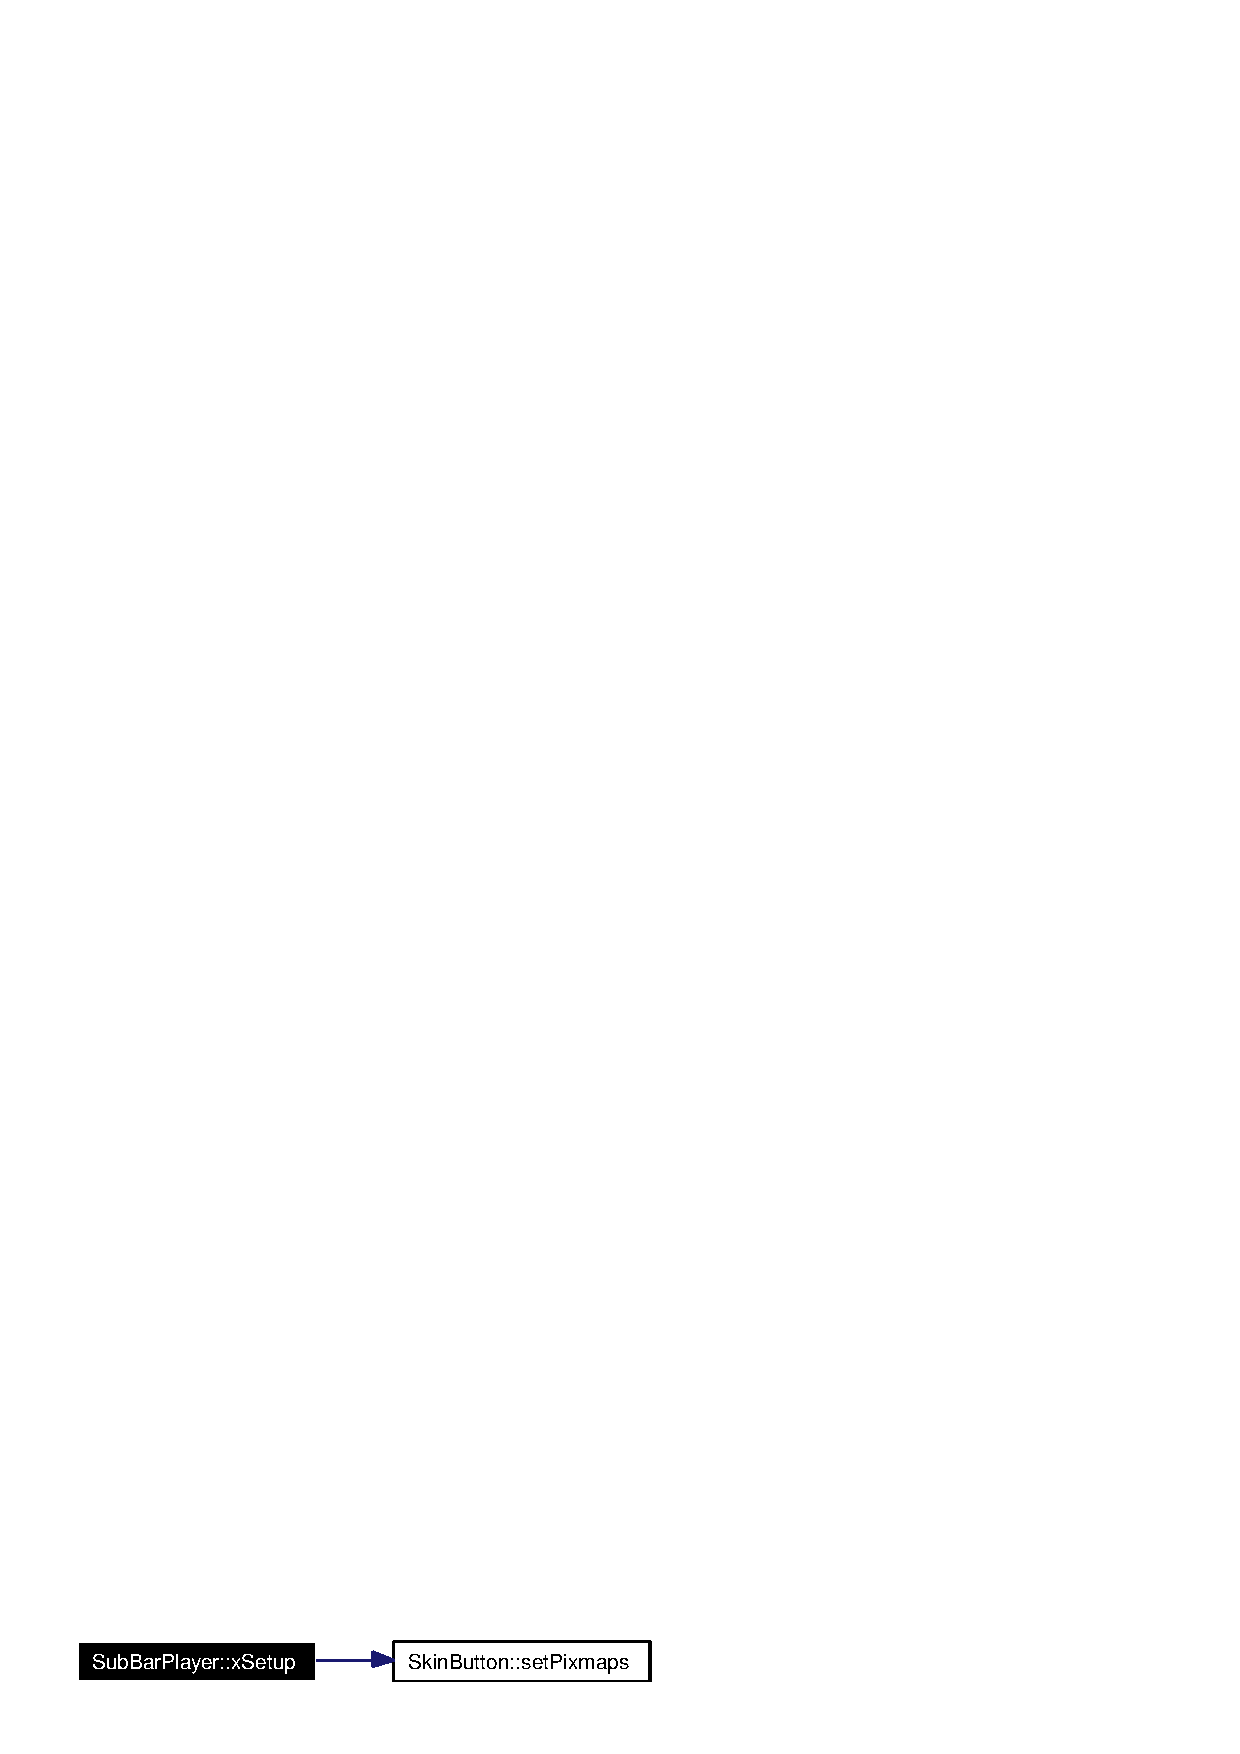
\includegraphics[width=156pt]{classSubBarPlayer_SubBarPlayera2_cgraph}
\end{center}
\end{figure}


\subsection{Member Data Documentation}
\index{SubBarPlayer@{Sub\-Bar\-Player}!backwardTimer@{backwardTimer}}
\index{backwardTimer@{backwardTimer}!SubBarPlayer@{Sub\-Bar\-Player}}
\subsubsection{\setlength{\rightskip}{0pt plus 5cm}QTimer$\ast$ {\bf Sub\-Bar\-Player::backward\-Timer}}\label{classSubBarPlayer_SubBarPlayero13}




Definition at line 52 of file subbarplayer.h.\index{SubBarPlayer@{Sub\-Bar\-Player}!backwardTimer@{backwardTimer}}
\index{backwardTimer@{backwardTimer}!SubBarPlayer@{Sub\-Bar\-Player}}
\subsubsection{\setlength{\rightskip}{0pt plus 5cm}QTimer$\ast$ {\bf Sub\-Bar\-Player::backward\-Timer}}\label{classSubBarPlayer_SubBarPlayero3}




Definition at line 52 of file src/subbarplayer.h.

Referenced by handle\-Previous\-Pressed(), handle\-Previous\-Released(), and x\-Setup().\index{SubBarPlayer@{Sub\-Bar\-Player}!BtnGraphic@{BtnGraphic}}
\index{BtnGraphic@{BtnGraphic}!SubBarPlayer@{Sub\-Bar\-Player}}
\subsubsection{\setlength{\rightskip}{0pt plus 5cm}QPixmap$\ast$ {\bf Sub\-Bar\-Player::Btn\-Graphic}[8]\hspace{0.3cm}{\tt  [private]}}\label{classSubBarPlayer_SubBarPlayerr4}




Definition at line 59 of file subbarplayer.h.\index{SubBarPlayer@{Sub\-Bar\-Player}!BtnGraphic@{BtnGraphic}}
\index{BtnGraphic@{BtnGraphic}!SubBarPlayer@{Sub\-Bar\-Player}}
\subsubsection{\setlength{\rightskip}{0pt plus 5cm}QPixmap$\ast$ {\bf Sub\-Bar\-Player::Btn\-Graphic}[8]\hspace{0.3cm}{\tt  [private]}}\label{classSubBarPlayer_SubBarPlayerr1}




Definition at line 59 of file src/subbarplayer.h.\index{SubBarPlayer@{Sub\-Bar\-Player}!forwardTimer@{forwardTimer}}
\index{forwardTimer@{forwardTimer}!SubBarPlayer@{Sub\-Bar\-Player}}
\subsubsection{\setlength{\rightskip}{0pt plus 5cm}QTimer$\ast$ {\bf Sub\-Bar\-Player::forward\-Timer}}\label{classSubBarPlayer_SubBarPlayero12}




Definition at line 51 of file subbarplayer.h.\index{SubBarPlayer@{Sub\-Bar\-Player}!forwardTimer@{forwardTimer}}
\index{forwardTimer@{forwardTimer}!SubBarPlayer@{Sub\-Bar\-Player}}
\subsubsection{\setlength{\rightskip}{0pt plus 5cm}QTimer$\ast$ {\bf Sub\-Bar\-Player::forward\-Timer}}\label{classSubBarPlayer_SubBarPlayero2}




Definition at line 51 of file src/subbarplayer.h.

Referenced by handle\-Next\-Pressed(), handle\-Next\-Released(), and x\-Setup().\index{SubBarPlayer@{Sub\-Bar\-Player}!m_pAnalyzer@{m\_\-pAnalyzer}}
\index{m_pAnalyzer@{m\_\-pAnalyzer}!SubBarPlayer@{Sub\-Bar\-Player}}
\subsubsection{\setlength{\rightskip}{0pt plus 5cm}{\bf QWidget}$\ast$ {\bf Sub\-Bar\-Player::m\_\-p\-Analyzer}}\label{classSubBarPlayer_SubBarPlayero10}




Definition at line 49 of file subbarplayer.h.\index{SubBarPlayer@{Sub\-Bar\-Player}!m_pAnalyzer@{m\_\-pAnalyzer}}
\index{m_pAnalyzer@{m\_\-pAnalyzer}!SubBarPlayer@{Sub\-Bar\-Player}}
\subsubsection{\setlength{\rightskip}{0pt plus 5cm}{\bf QWidget}$\ast$ {\bf Sub\-Bar\-Player::m\_\-p\-Analyzer}}\label{classSubBarPlayer_SubBarPlayero0}




Definition at line 49 of file src/subbarplayer.h.\index{SubBarPlayer@{Sub\-Bar\-Player}!m_player@{m\_\-player}}
\index{m_player@{m\_\-player}!SubBarPlayer@{Sub\-Bar\-Player}}
\subsubsection{\setlength{\rightskip}{0pt plus 5cm}{\bf Myplayer}$\ast$ {\bf Sub\-Bar\-Player::m\_\-player}}\label{classSubBarPlayer_SubBarPlayero14}




Definition at line 53 of file subbarplayer.h.\index{SubBarPlayer@{Sub\-Bar\-Player}!m_player@{m\_\-player}}
\index{m_player@{m\_\-player}!SubBarPlayer@{Sub\-Bar\-Player}}
\subsubsection{\setlength{\rightskip}{0pt plus 5cm}{\bf Myplayer}$\ast$ {\bf Sub\-Bar\-Player::m\_\-player}}\label{classSubBarPlayer_SubBarPlayero4}




Definition at line 53 of file src/subbarplayer.h.

Referenced by handle\-Next\-Released(), handle\-Previous\-Released(), handle\-Slider\-Released(), init\-Media(), insert\-Media(), remove\-Media(), Sub\-Bar\-Player(), x\-Setup(), HDASS08::x\-Setup(), and $\sim$Sub\-Bar\-Player().\index{SubBarPlayer@{Sub\-Bar\-Player}!pixBackground@{pixBackground}}
\index{pixBackground@{pixBackground}!SubBarPlayer@{Sub\-Bar\-Player}}
\subsubsection{\setlength{\rightskip}{0pt plus 5cm}QPixmap {\bf Sub\-Bar\-Player::pix\-Background}\hspace{0.3cm}{\tt  [private]}}\label{classSubBarPlayer_SubBarPlayerr0}




Definition at line 58 of file subbarplayer.h.\index{SubBarPlayer@{Sub\-Bar\-Player}!playerPosition@{playerPosition}}
\index{playerPosition@{playerPosition}!SubBarPlayer@{Sub\-Bar\-Player}}
\subsubsection{\setlength{\rightskip}{0pt plus 5cm}QSlider$\ast$ {\bf Sub\-Bar\-Player::player\-Position}}\label{classSubBarPlayer_SubBarPlayero11}




Definition at line 50 of file subbarplayer.h.\index{SubBarPlayer@{Sub\-Bar\-Player}!playerPosition@{playerPosition}}
\index{playerPosition@{playerPosition}!SubBarPlayer@{Sub\-Bar\-Player}}
\subsubsection{\setlength{\rightskip}{0pt plus 5cm}QSlider$\ast$ {\bf Sub\-Bar\-Player::player\-Position}}\label{classSubBarPlayer_SubBarPlayero1}




Definition at line 50 of file src/subbarplayer.h.

Referenced by handle\-Backward(), handle\-Forward(), handle\-Message(), handle\-Next\-Released(), handle\-Position(), handle\-Previous\-Released(), handle\-Slider\-Released(), and x\-Setup().\index{SubBarPlayer@{Sub\-Bar\-Player}!receive_list@{receive\_\-list}}
\index{receive_list@{receive\_\-list}!SubBarPlayer@{Sub\-Bar\-Player}}
\subsubsection{\setlength{\rightskip}{0pt plus 5cm}KURL::List {\bf Sub\-Bar\-Player::receive\_\-list}}\label{classSubBarPlayer_SubBarPlayero5}




Definition at line 54 of file subbarplayer.h.

Referenced by slot\-Receive\-PL().\index{SubBarPlayer@{Sub\-Bar\-Player}!slider@{slider}}
\index{slider@{slider}!SubBarPlayer@{Sub\-Bar\-Player}}
\subsubsection{\setlength{\rightskip}{0pt plus 5cm}bool {\bf Sub\-Bar\-Player::slider}\hspace{0.3cm}{\tt  [private]}}\label{classSubBarPlayer_SubBarPlayerr3}




Definition at line 61 of file subbarplayer.h.

Referenced by handle\-Next\-Pressed(), handle\-Next\-Released(), handle\-Position(), handle\-Previous\-Pressed(), handle\-Previous\-Released(), handle\-Slider\-Pressed(), handle\-Slider\-Released(), and Sub\-Bar\-Player().\index{SubBarPlayer@{Sub\-Bar\-Player}!state@{state}}
\index{state@{state}!SubBarPlayer@{Sub\-Bar\-Player}}
\subsubsection{\setlength{\rightskip}{0pt plus 5cm}{\bf PLAYSTATE} {\bf Sub\-Bar\-Player::state}\hspace{0.3cm}{\tt  [private]}}\label{classSubBarPlayer_SubBarPlayerr2}




Definition at line 60 of file subbarplayer.h.\index{SubBarPlayer@{Sub\-Bar\-Player}!SubBtn_Forward@{SubBtn\_\-Forward}}
\index{SubBtn_Forward@{SubBtn\_\-Forward}!SubBarPlayer@{Sub\-Bar\-Player}}
\subsubsection{\setlength{\rightskip}{0pt plus 5cm}{\bf Skin\-Button} $\ast$ {\bf Sub\-Bar\-Player::Sub\-Btn\_\-Forward}}\label{classSubBarPlayer_SubBarPlayero8}




Definition at line 55 of file subbarplayer.h.

Referenced by x\-Setup().\index{SubBarPlayer@{Sub\-Bar\-Player}!SubBtnPlayer_Backword@{SubBtnPlayer\_\-Backword}}
\index{SubBtnPlayer_Backword@{SubBtnPlayer\_\-Backword}!SubBarPlayer@{Sub\-Bar\-Player}}
\subsubsection{\setlength{\rightskip}{0pt plus 5cm}{\bf Skin\-Button} $\ast$ {\bf Sub\-Bar\-Player::Sub\-Btn\-Player\_\-Backword}}\label{classSubBarPlayer_SubBarPlayero7}




Definition at line 55 of file subbarplayer.h.

Referenced by x\-Setup().\index{SubBarPlayer@{Sub\-Bar\-Player}!SubBtnPlayer_PlayNPause@{SubBtnPlayer\_\-PlayNPause}}
\index{SubBtnPlayer_PlayNPause@{SubBtnPlayer\_\-PlayNPause}!SubBarPlayer@{Sub\-Bar\-Player}}
\subsubsection{\setlength{\rightskip}{0pt plus 5cm}{\bf Skin\-Button}$\ast$ {\bf Sub\-Bar\-Player::Sub\-Btn\-Player\_\-Play\-NPause}}\label{classSubBarPlayer_SubBarPlayero15}




Definition at line 55 of file subbarplayer.h.\index{SubBarPlayer@{Sub\-Bar\-Player}!SubBtnPlayer_PlayNPause@{SubBtnPlayer\_\-PlayNPause}}
\index{SubBtnPlayer_PlayNPause@{SubBtnPlayer\_\-PlayNPause}!SubBarPlayer@{Sub\-Bar\-Player}}
\subsubsection{\setlength{\rightskip}{0pt plus 5cm}{\bf Skin\-Button}$\ast$ {\bf Sub\-Bar\-Player::Sub\-Btn\-Player\_\-Play\-NPause}}\label{classSubBarPlayer_SubBarPlayero6}




Definition at line 55 of file src/subbarplayer.h.

Referenced by Change\-Btn\-Play\-Pause\-Graphic(), and x\-Setup().\index{SubBarPlayer@{Sub\-Bar\-Player}!testBtn@{testBtn}}
\index{testBtn@{testBtn}!SubBarPlayer@{Sub\-Bar\-Player}}
\subsubsection{\setlength{\rightskip}{0pt plus 5cm}{\bf Skin\-Button} $\ast$ {\bf Sub\-Bar\-Player::test\-Btn}}\label{classSubBarPlayer_SubBarPlayero9}




Definition at line 55 of file subbarplayer.h.

The documentation for this class was generated from the following files:\begin{CompactItemize}
\item 
{\bf src/subbarplayer.h}\item 
{\bf subbarplayer.h}\item 
{\bf subbarplayer.moc}\item 
{\bf src/subbarplayer.cpp}\item 
{\bf subbarplayer.cpp}\end{CompactItemize}
